\documentclass{bhcguides}

\usepackage[a4paper, portrait, margin=1.2in]{geometry}
\usepackage[utf8]{inputenc}
\usepackage{tabu}
\setlength{\parindent}{0pt}
\setlength{\parskip}{6 pt}

\usepackage{graphicx}
\graphicspath{ {images/} }

\usepackage{url}
\usepackage{hyperref}
\usepackage{cite}

\begin{document}

\title{Administrator Manual}

\includegraphics[width=1.0\textwidth]{BHCbanner.png}
\date{\today}
\maketitle

\tableofcontents
\pagebreak

\section{Overview}

The Building Healthy Communities programme is a partnership that delivers a range of initiatives, activites, interventions and skills classes to improve the wellbeing of the community as a whole, and the members of that community. As an administrator, you have access to the inner workings of the system, to view and collate metrics on how well the programme is running, and the ability to create and manage initiatives across the Area Partnerships. But if you've come this far, you already know that. What you want to know is, what's this website got to do with anything, and how do I use it? That's where this manual comes in.

The Building Healthy Communities web system is a way to give you, the administrator, the power to easily and simply manage all the data driven aspects of the BHC programme from one consistent location. The service users and volunteers each use other sections of the system, with all their data feeding through to you, where you can view it in the manner you wish. Data can be viewed from the initiative level, through funding, all the way down to the details of individual service users and volunteers, and can be viewed in tables, searched, and downloaded for use elsewhere. Feedback is also integrated into the system, allowing you to track the efficacy of initiatives and the welfare of service users. This manual will walk you through the use of the system, and introduce you to the various features and intricacies of the system, giving examples as we go.

\pagebreak

\section{System Access and Login}
\label{sec:syslogin}

The system is currently hosted can be accessed through most major web browsers (Chrome, Firefox, Safari, IE8 or higher). Before accessing the system, you should have your email address and password on hand. If you are a new administrator, who has not previously accessed the system, you should ask another administrator to create an account for you. Upon entering the system, you will be taken to the login page, as seen in \autoref{fig:initialLogin}.

\begin{figure}[h!]
 \centerline{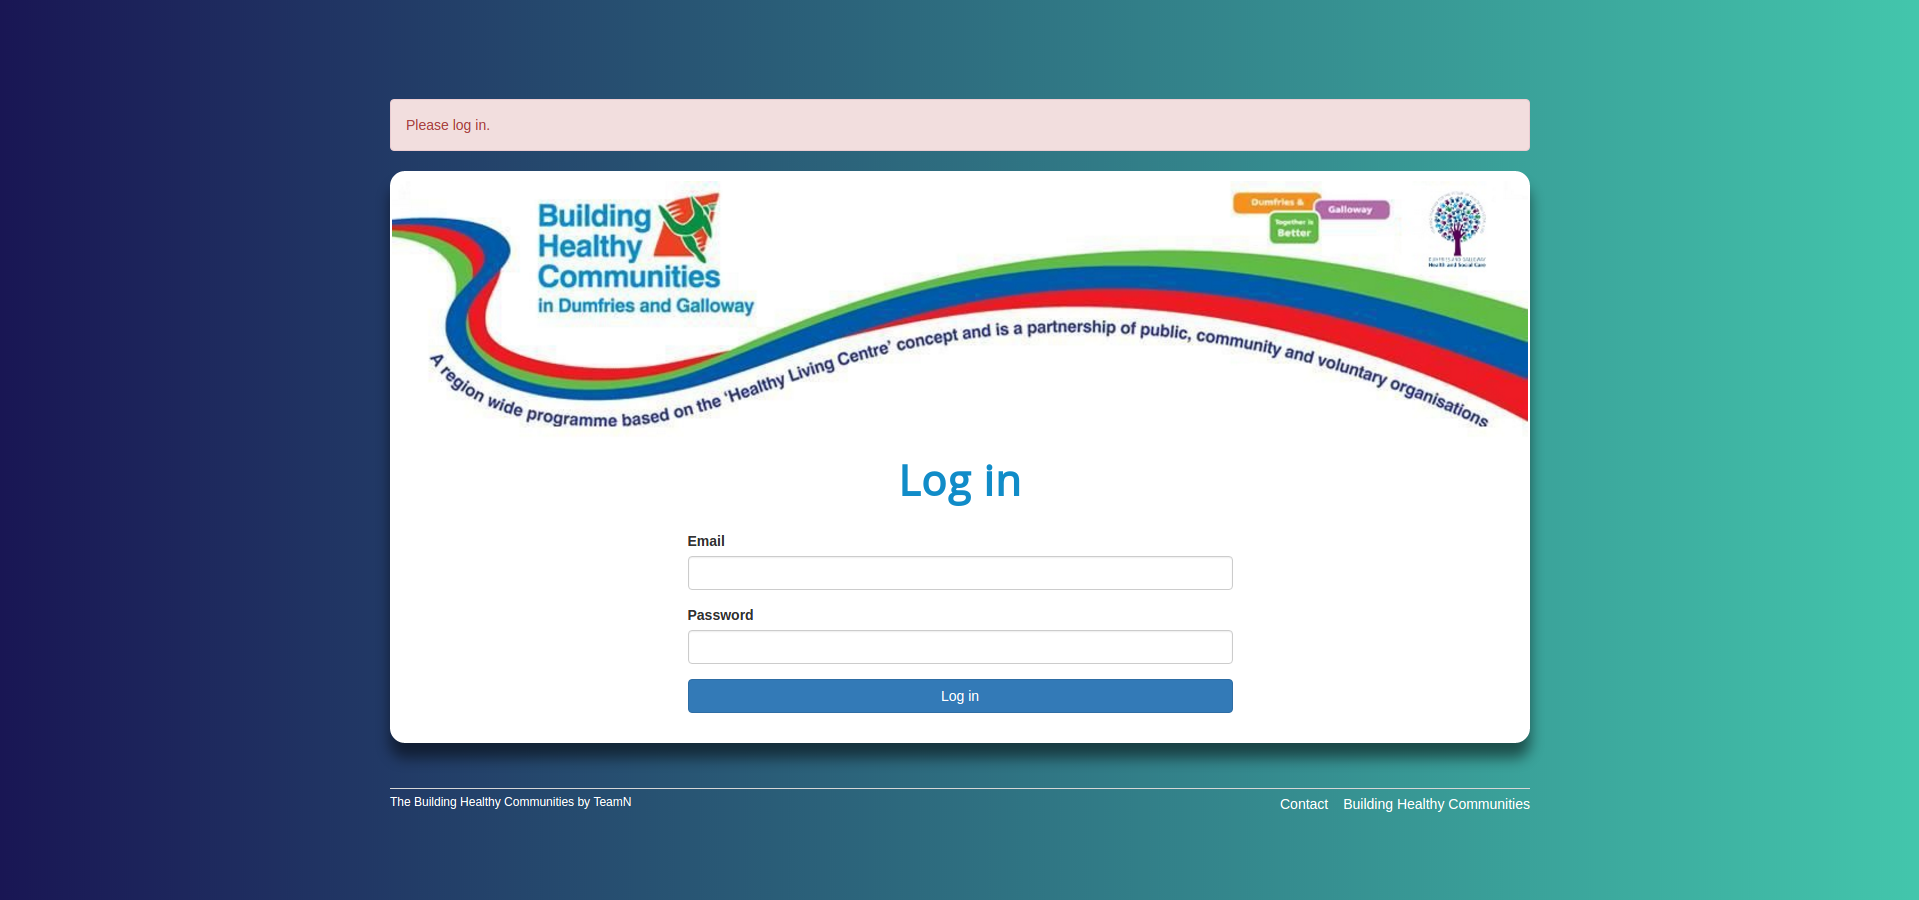
\includegraphics[width=\textwidth, height=\textheight, keepaspectratio]{loginscreen.png}}
 \caption{Login page}
 \label{fig:initialLogin}
\end{figure}

To login to the system, enter your email address and password. Until you do so, there is no way to gain access beyond this page. In the case that you have forgotten your email address and/or password, see \autoref{sec:contacts}: Contacts and Forgotten Passwords.

\section{Menu Bar}
\label{sec:menubar}

The menu bar is a persistent feature, appearing at the top of every page on the system. It is designed to allow quick access to every major area of the site, combining a collection of quick links to commonly used sections with a menu bar containing links to the other sections. There is also a Log out button that will log you out and return you to the login screen.

\begin{figure}[h!]
 \centerline{
\includegraphics[width=\textwidth, height=\textheight, keepaspectratio]{menubar.png}}
 \caption{Menu bar with drop down}
 \label{fig:initialLogin}
\end{figure}
\pagebreak

\section{Home Page}
\label{sec:homepage}

Upon logging in to the system, the first page that will be loaded is the home page. This page is a quick overview of the system, presenting groups of useful information and allowing you to quickly navigate and execute a few simple actions. The home page is split into three sections: the Area Overview, Statistics, and Service Requests.

\subsection{Area Overview}
\label{ssec:areaoverview}

The Area Overview is the first major feature on the website home page. From here you can quickly see the names of every initiative run by each area partnership. Clicking the name of an area will take you the relevant area page, and clicking an initiative name will do so for relevant initiative. For more information on areas and initiatives see \autoref{sec:areas}: Areas and \autoref{sec:initiatives}: Initiatives.

\begin{figure}[h!]
 \centerline{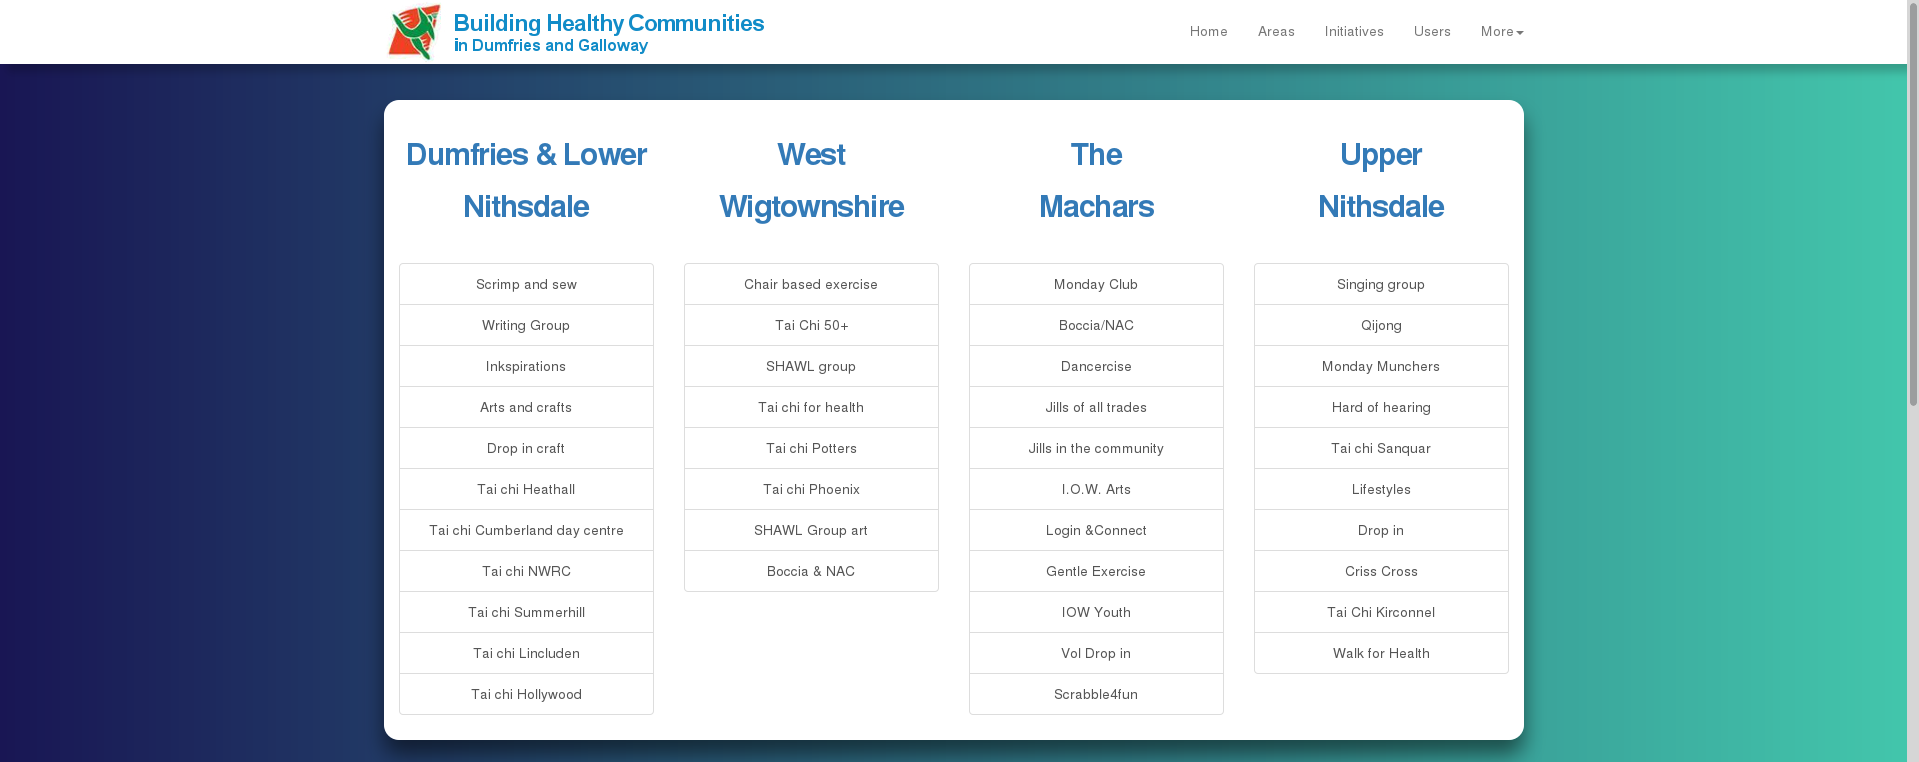
\includegraphics[width=\textwidth, height=\textheight, keepaspectratio]{homepage1.png}}
 \caption{Area Overview}
 \label{fig:homePage1}
\end{figure}

\subsection{Statistics}
\label{ssec:statistics}

The Statistics section is a quick rundown of the status of the system as a whole. It features a small collection of information, including:

\begin{itemize}
	\item The total number of service users, volunteers, and funders
	\item The most and least popular initiatives (those with the highest and lowest number of members)
	\item The most and least assigned medical conditions
	\item A graph of the total monthly attendance across all initiatives over the last 2 years
	\item A graph of the average monthly attendance as a percentage, over the same period as above.
\end{itemize}

Clicking the name of an initiative or condition will take you to the relevant details page.

\begin{figure}[h!]
 \centerline{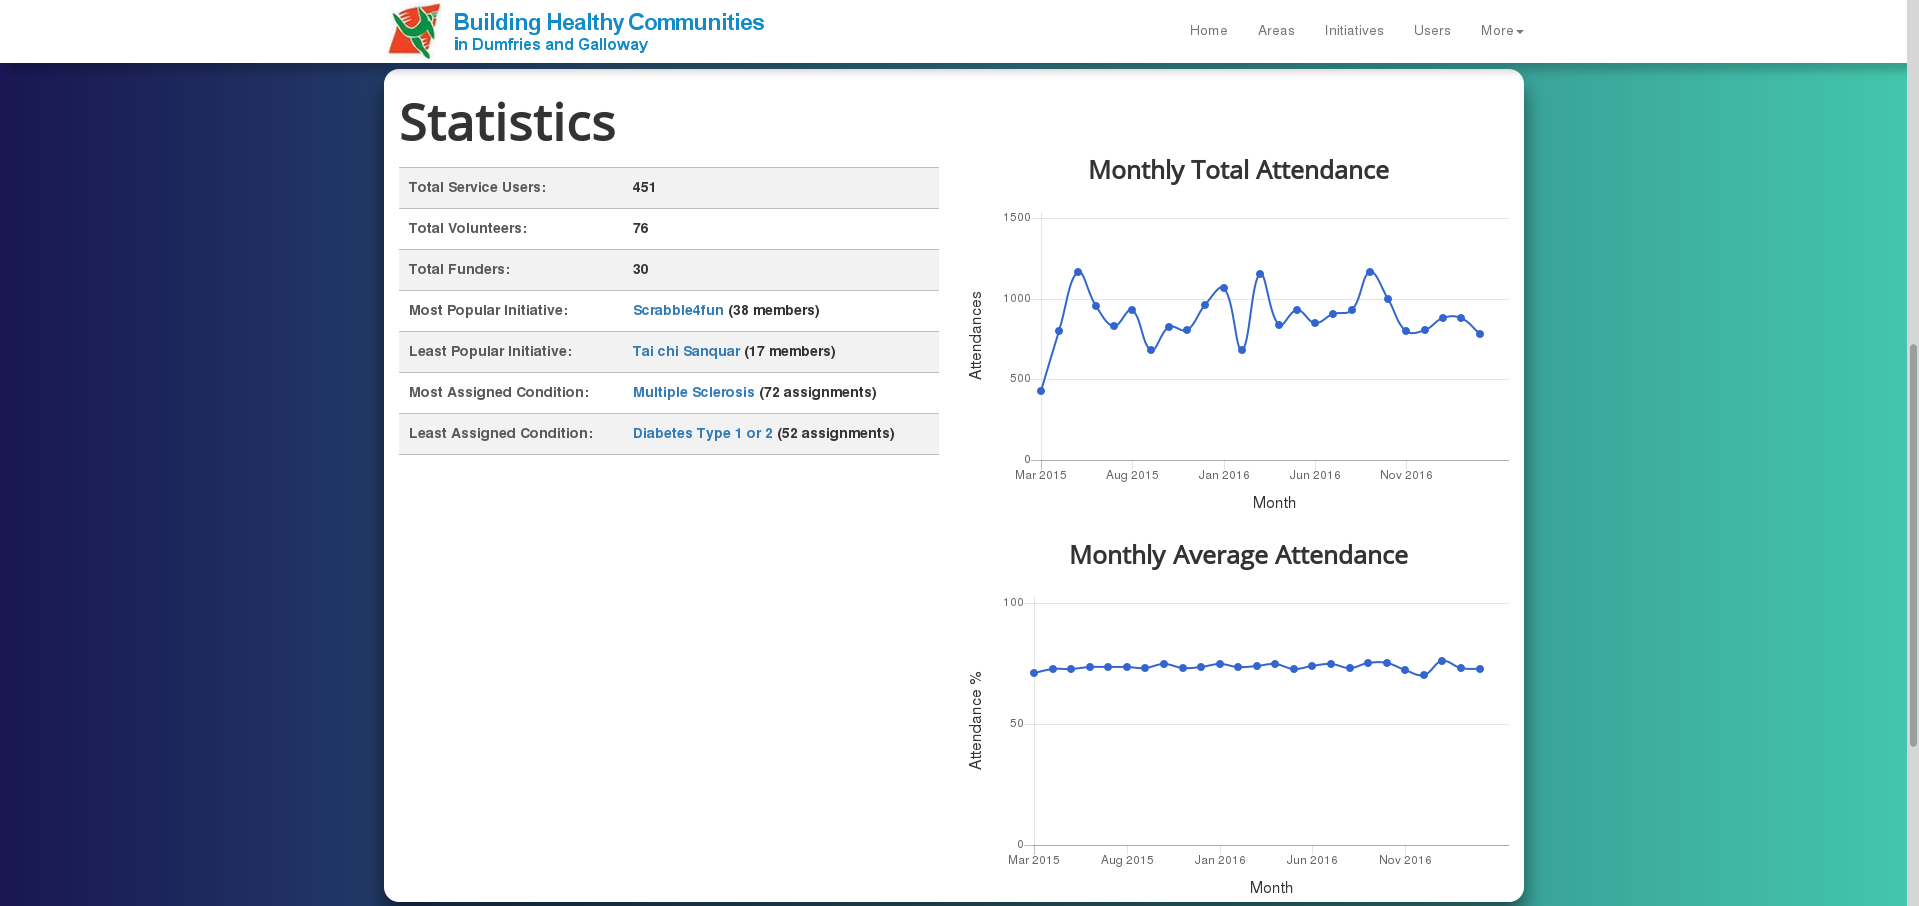
\includegraphics[width=\textwidth, height=\textheight, keepaspectratio]{homepage2.png}}
 \caption{Statistics}
 \label{fig:statistics}
\end{figure}

\subsection{Service Requests}
\label{ssec:servicerequests}

The service requests section allows you to see all the messages sent to you by service users ad volunteers asking you to change their details. To change their details, open the user's profile, change the relevant details (described in more details in \autoref{sec:users}: Users, and save them. You can then delete the service request.

\begin{figure}[h!]
 \centerline{
\includegraphics[width=\textwidth, height=\textheight, keepaspectratio]{homepage3.png}}
 \caption{Service Requests}
 \label{fig:serviceRequests}
\end{figure}

\pagebreak

\section{Data Tables}
\label{sec:datatables}

The data tables are the main focus of the system, the 'power tabs', so to speak. From these pages, you can browse all the entries in the system, or query the database to find specific data. The data tables can be accessed by clicking the relevant link in the menu bar; for example, to get to the Initiatives data table, click the 'Initiatives' link. 

\subsection{Browsing and Organising}
\label{ssec:browsingtables}

To browse a table, simply scroll down the page to view more results. There are 30 results displayed per page, and more can be loaded by clicking the 'next' button or a number at the bottom of the page. The tables can also be organised by any of the columns; clicking the up or down arrow in a column will sort the table by that column in ascending or descending order respectively. \autoref{fig:initAscName} shows the second page of the Initiatives table ranked in ascending order by name.

\begin{figure}[h!]
 \centerline{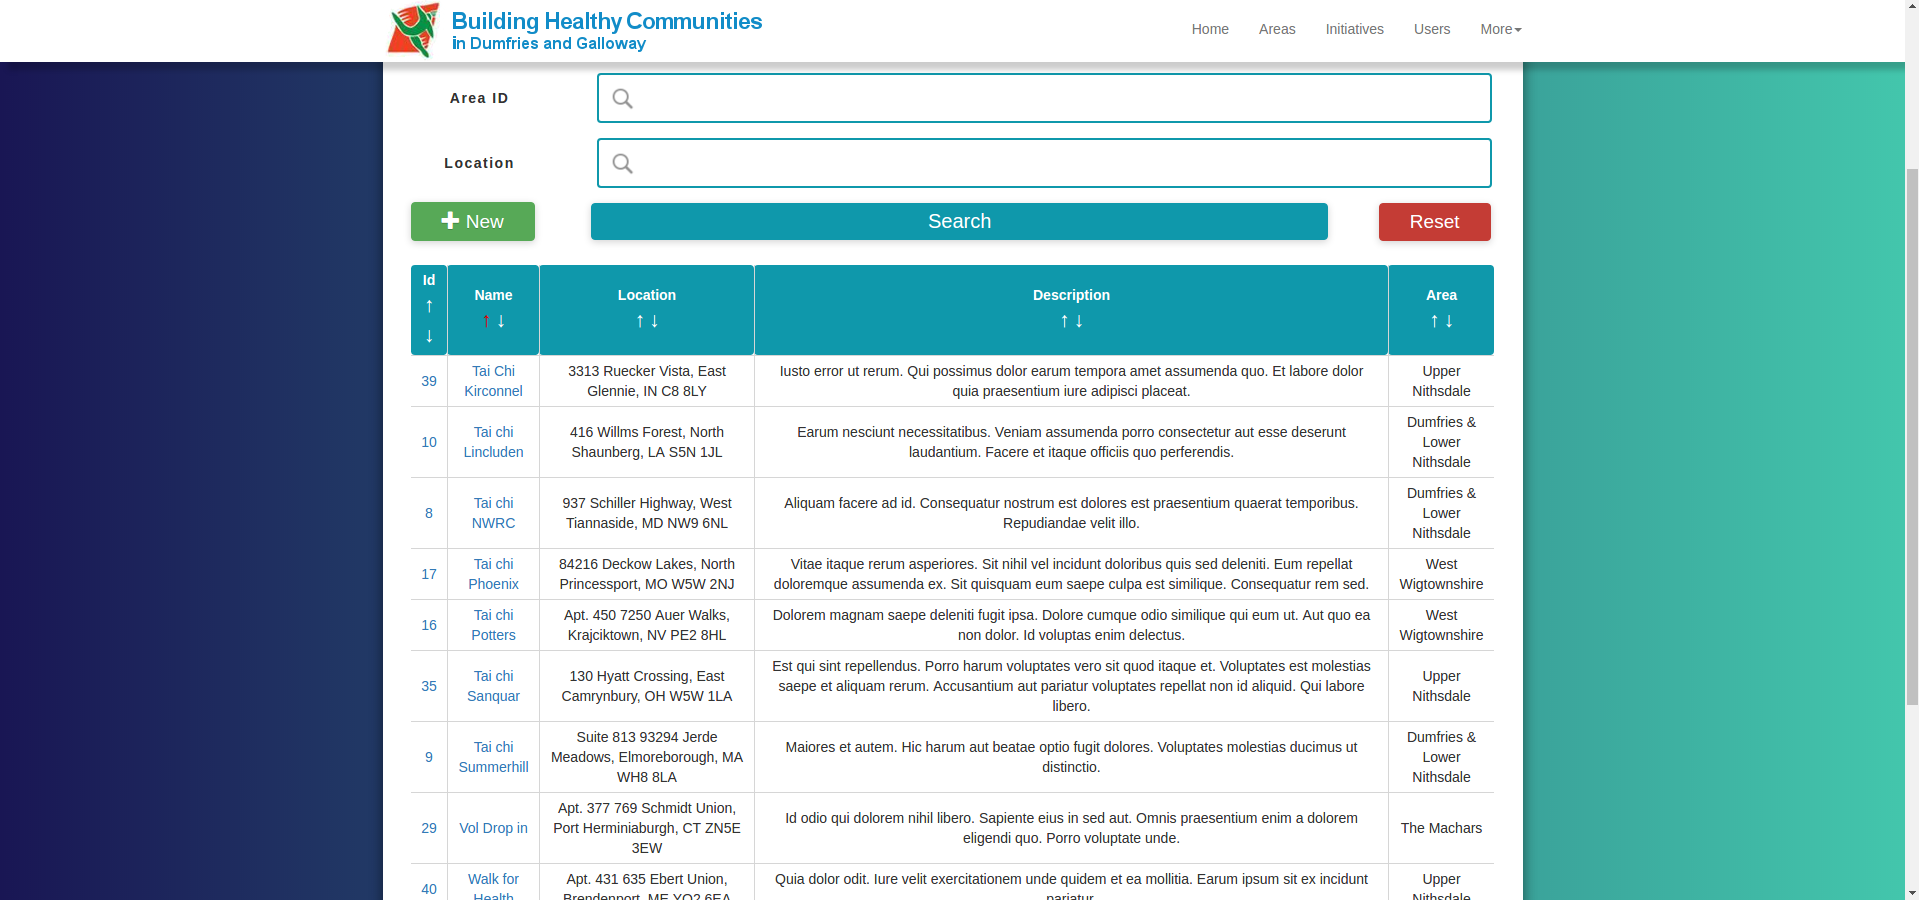
\includegraphics[width=\textwidth, height=\textheight, keepaspectratio]{initiativesnameascending.png}}
 \caption{Second page of initiatives ranked in ascending name order}
 \label{fig:initAscName}
\end{figure}

\subsection{Querying}
\label{ssec:search}

The data tables can also be queries by each column. To query a table, type your query into the relevant search box, and click search. The boxes are not case sensitive, so 'TAI' and 'tai', or even 'tAi' will return the same results. Queries can also be partial matches, so a search for the number '0141' in a telephone field for example would return every result with a phone number containing those numbers. Incorrect spellings however, are not corrected, so a search for 'Thai' when you intended to search for 'Tai' will not return any results relating to 'Tai'. It is also possible to query multiple columns at once. In \autoref{fig:initSearch}), there is an example of the result of searching for all 'Tai' events in a location containing the word 'North'. Queries can be reset by clicking the red 'Reset' button to the right of the search button.

\begin{figure}[h!]
 \centerline{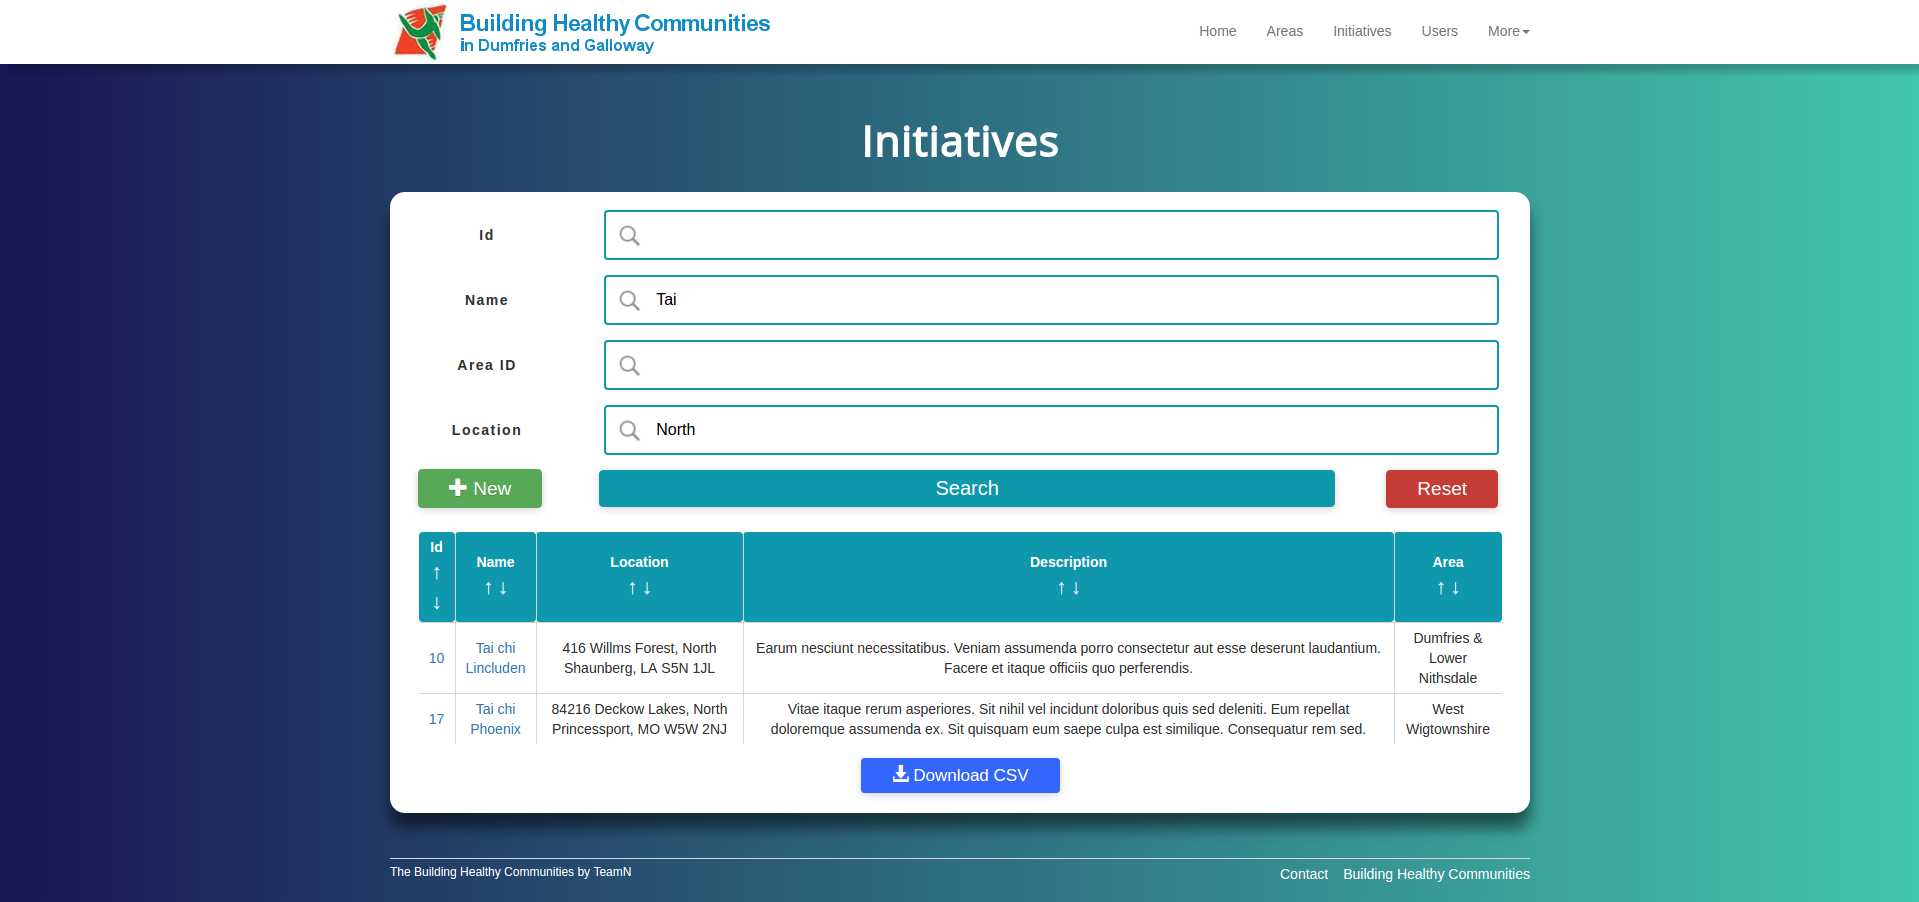
\includegraphics[width=\textwidth, height=\textheight, keepaspectratio]{initsearch.png}}
 \caption{Initiative search for 'Tai' and 'North'}
 \label{fig:initSearch}
\end{figure}

\subsection{Downloading}
\label{ssec:download}

It is possible to download the result of any query in the Areas, Initiatives, and Users tables. To do so, scroll to the bottom of the table and click the blue 'Download CSV' button, seen in \autoref{fig:download}. This will download a CSV file, compatible with spreadsheet software such as Microsoft Excel. It is also possible to download the contents of an entire table without querying, by clicking download without entering a query.

\begin{figure}[h!]
 \centerline{
\includegraphics[width=\textwidth, height=\textheight, keepaspectratio]{downloadbutton.png}}
 \caption{Download Button}
 \label{fig:download}
\end{figure}

\subsection{Adding New Entries}
\label{ssec:addentries}

The final feature available on the data table pages is the ability to add a new entry to the table. The content of a new entry varies by table, but the method is always the same. To add a new entry, click the green 'New Entry' button to the left of the search button. This will take you to the relevant new entry screen. The example in \autoref{fig:newUser} shows a new user being added to the Users table. For more information on the full content of an entry, see the relevant section of the guide.

\begin{figure}[h!]
 \centerline{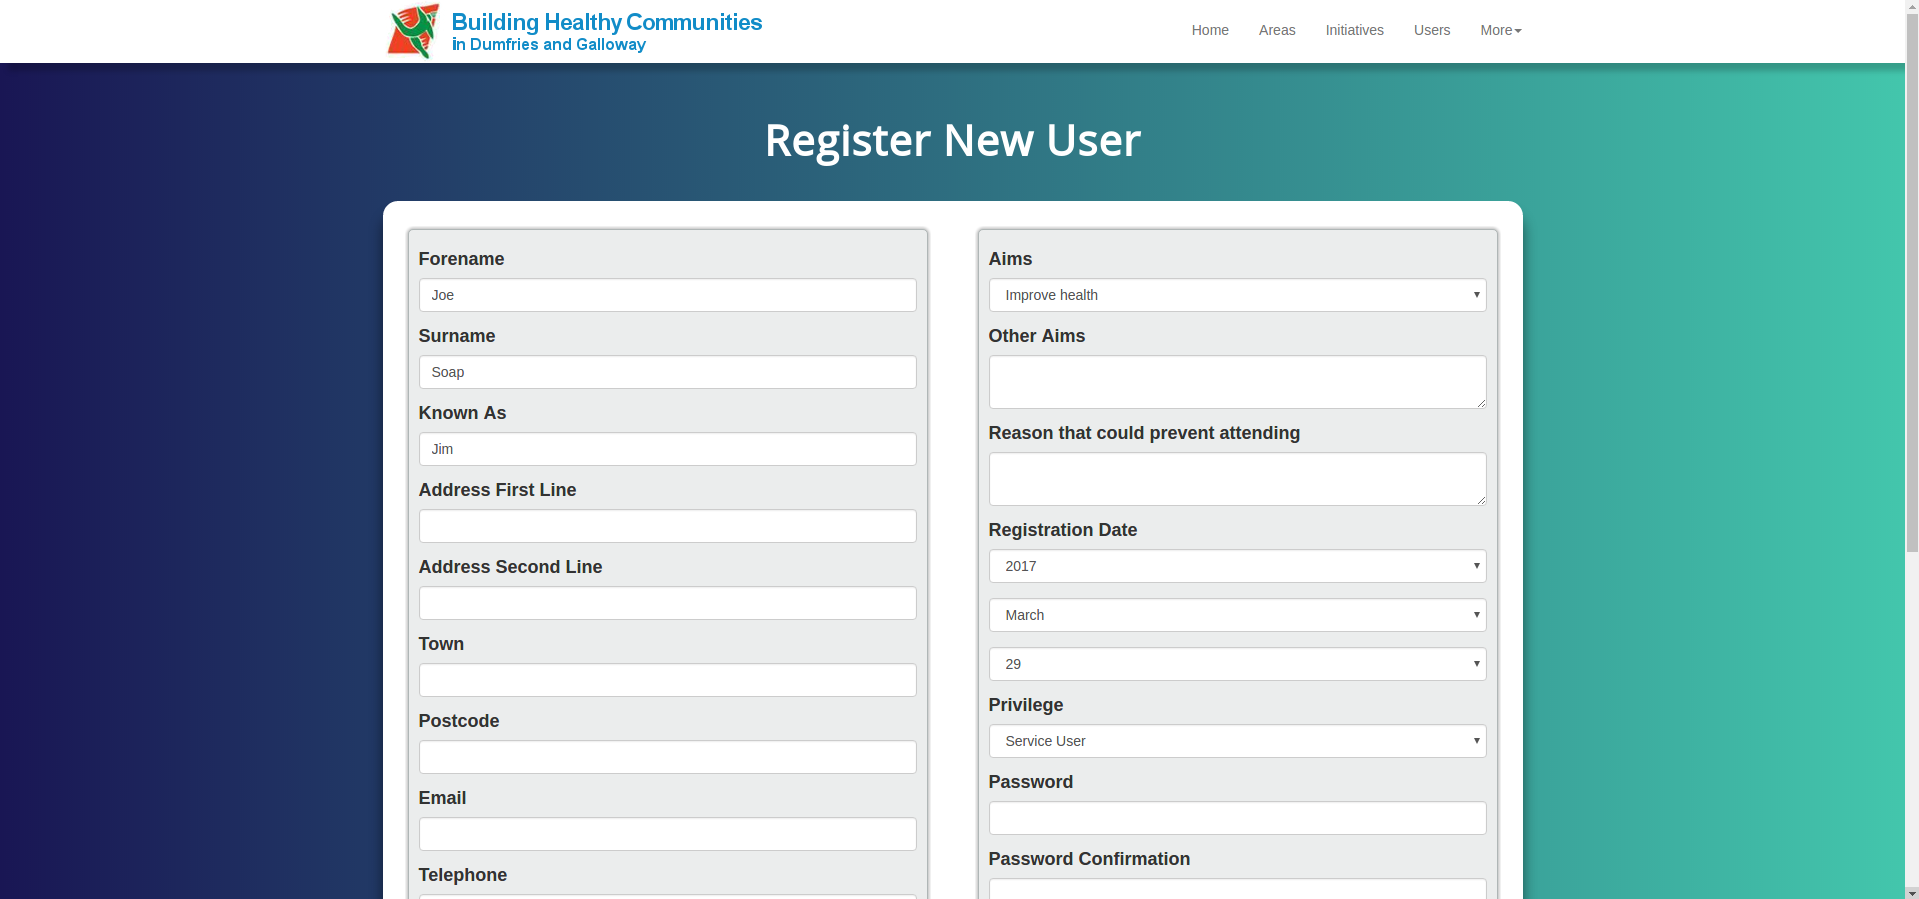
\includegraphics[width=\textwidth, height=\textheight, keepaspectratio]{newuser.png}}
 \caption{Adding a new user}
 \label{fig:newUser}
\end{figure}

\pagebreak

\section{Areas}
\label{sec:areas}

Areas are the largest unit in the Building Healthy Communities programme, being the geographic regions in which initiatives take place. To access the main page of an area, click its name anywhere in the system where it is in blue text. The easiest places to find a link such as this are the Area table, and the links on the home page.

\subsection{Information and Statistics}
\label{ssec:areainfoandstats}

The main page for an area consists of all the information pertaining to that area laid out in three sections:

\begin{itemize}
	\item The first section contains the area's name, a brief description, the numbers of initiatives active in the area and the number of users enrolled in those initiatives. It also contains a graph of the number of users per initiative.
	\item The second section contains a table listing all the initiatives for the area. It can be organised by column the same way as the data tables, but not searched.
	\item The third section contains another table, this time listing all the users enrolled in initiatives within the area. Again, it can be organised but not searched.
\end{itemize}

\begin{figure}[h]
 \centerline{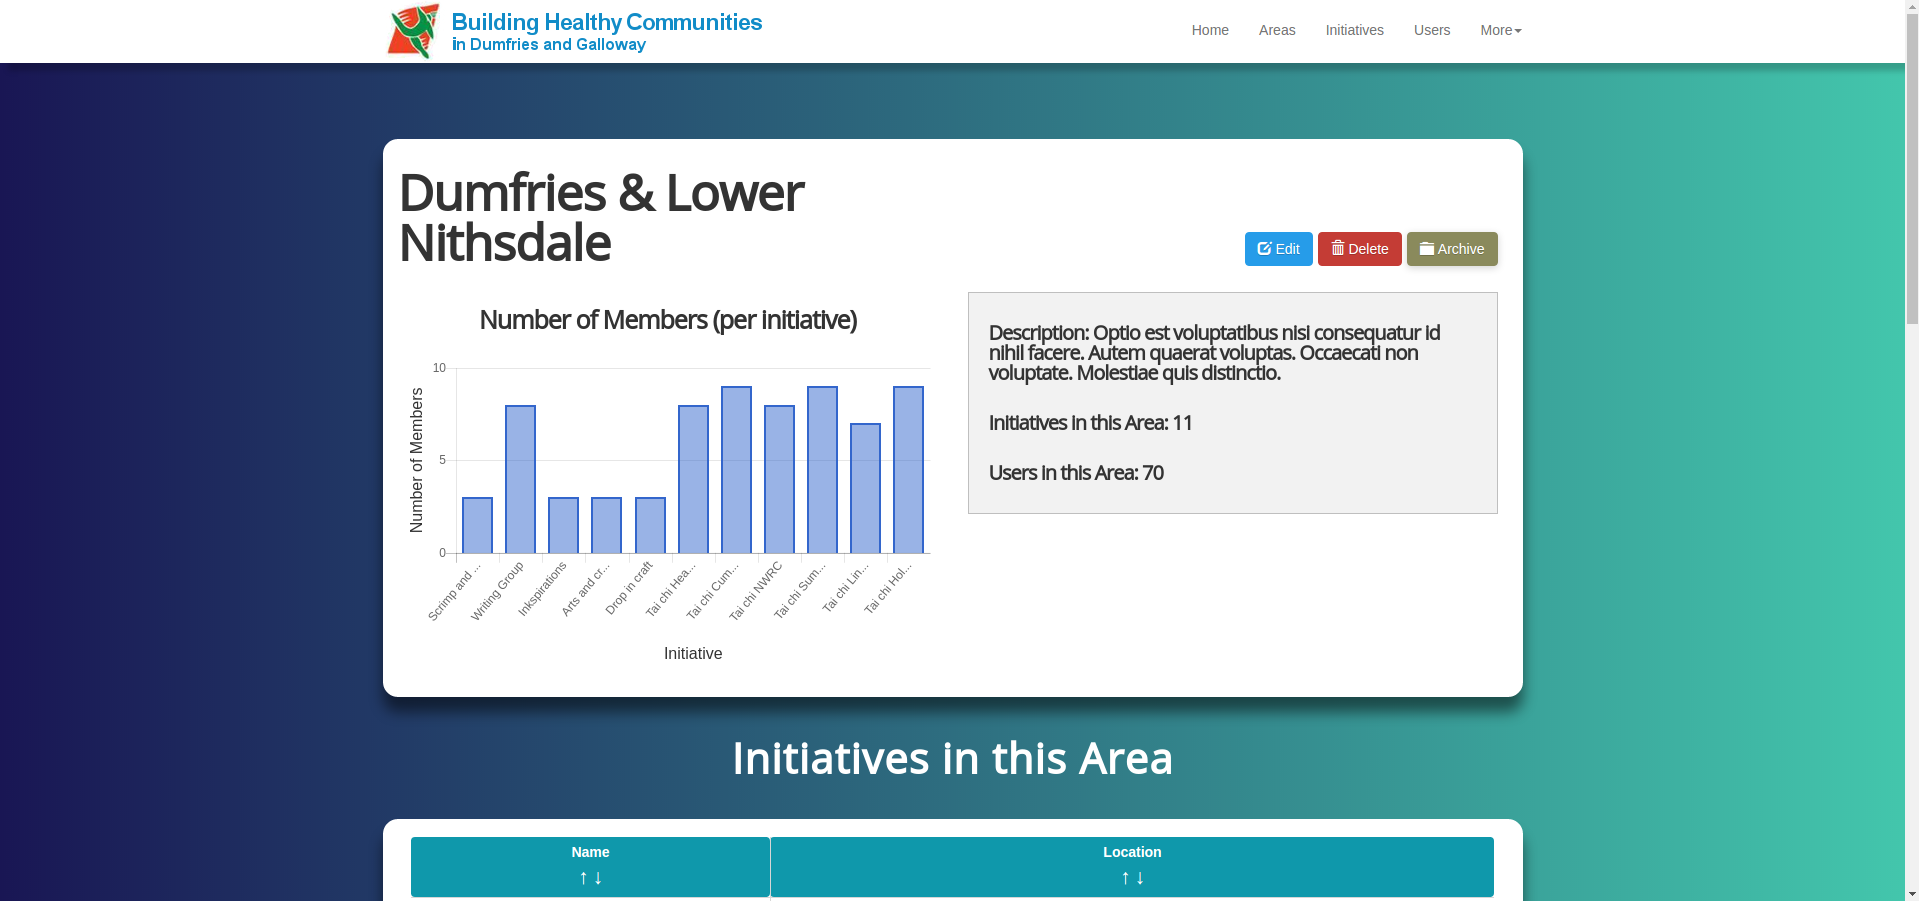
\includegraphics[width=\textwidth, height=\textheight, keepaspectratio]{areamainpage.png}}
 \caption{Area Main Page}
 \label{fig:areaMainPage}
\end{figure}

\subsection{Editing, Deleting and Archiving}
\label{ssec:areaeditdelete}

The only actions that can be taken with an existing area are editing its details, deleting it, or archiving it. The buttons for all three actions are placed next to each other, above the information box.

Editing the area allows you to change its name and description. As an area is effectively just a geographic region in which other things happen, there is no other information to change. The editing screen can be seen in \autoref{fig:areaEdit}.

Deleting an area will permanently delete it from the database. Any associated initiatives will also be permanently deleted, and those initiatives will disappear from the enrolment lists of each user that was enrolled in them. This is a permanent action, deleting the data itself, and cannot be undone!

Archiving an area is similar to deleting, except that it will not permanently delete data. Instead, the area and its initiatives will be placed in the archives. For more on archiving, see \autoref{sec:archives}

\begin{figure}[h!]
 \centerline{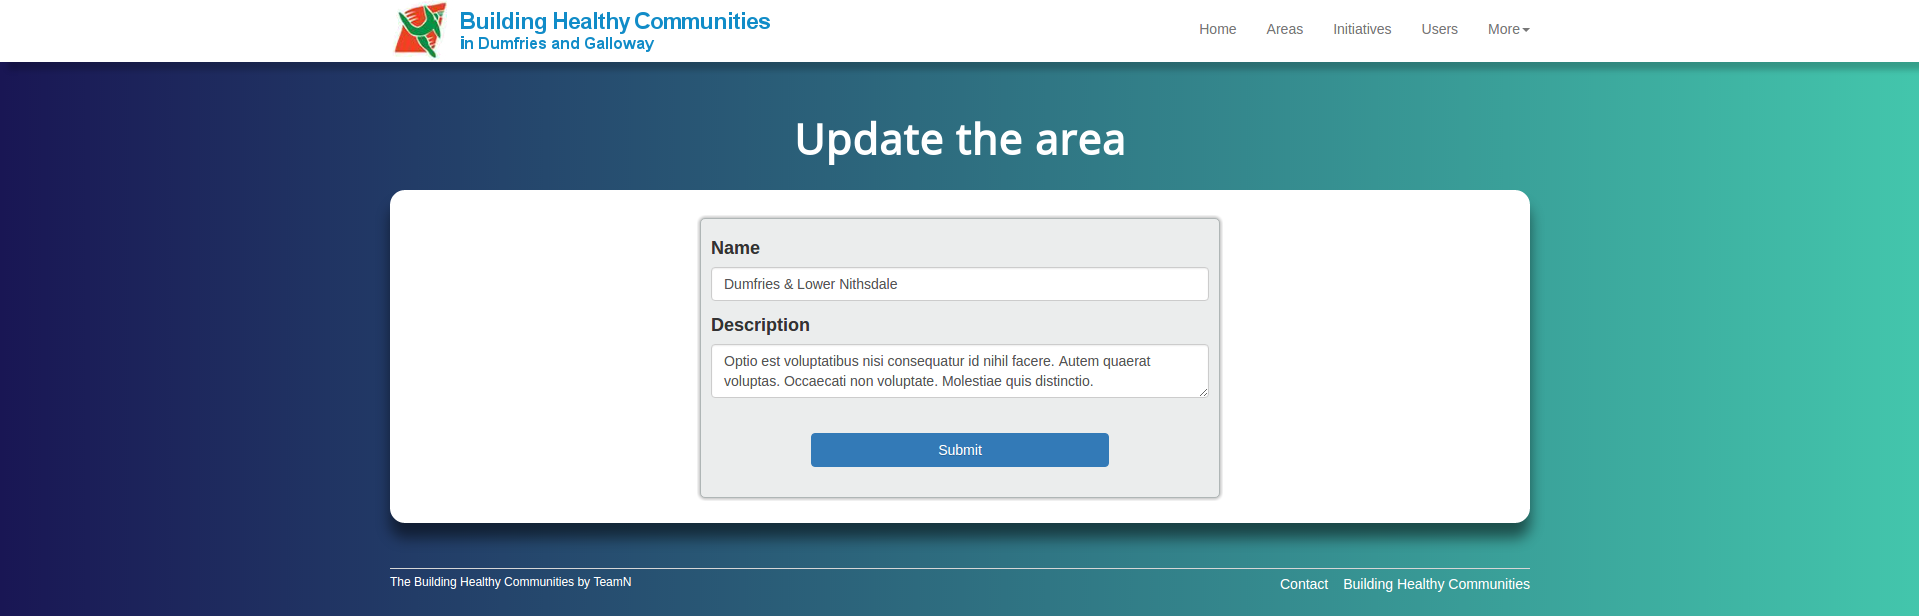
\includegraphics[width=\textwidth, height=\textheight, keepaspectratio]{areaedit.png}}
 \caption{Editing an area}
 \label{fig:areaEdit}
\end{figure}

\subsection{Creating a New Area}
\label{ssec:createarea}

To create a new area, you must click the 'New' button on the Area data table page, as described in \autoref{sec:datatables}: Data Tables, and you will be taken to a short area creation screen, as seen in \autoref{fig:createArea}. As with the edit option, adding a name and description is all that is necessary to create an area. The newly created area will have no initiatives, and therefore no users either. To see how to assign users and initiatives to an area, see \autoref{sec:initiatives}: Initiatives and \autoref{sec:users}: Users.

\begin{figure}[h!]
 \centerline{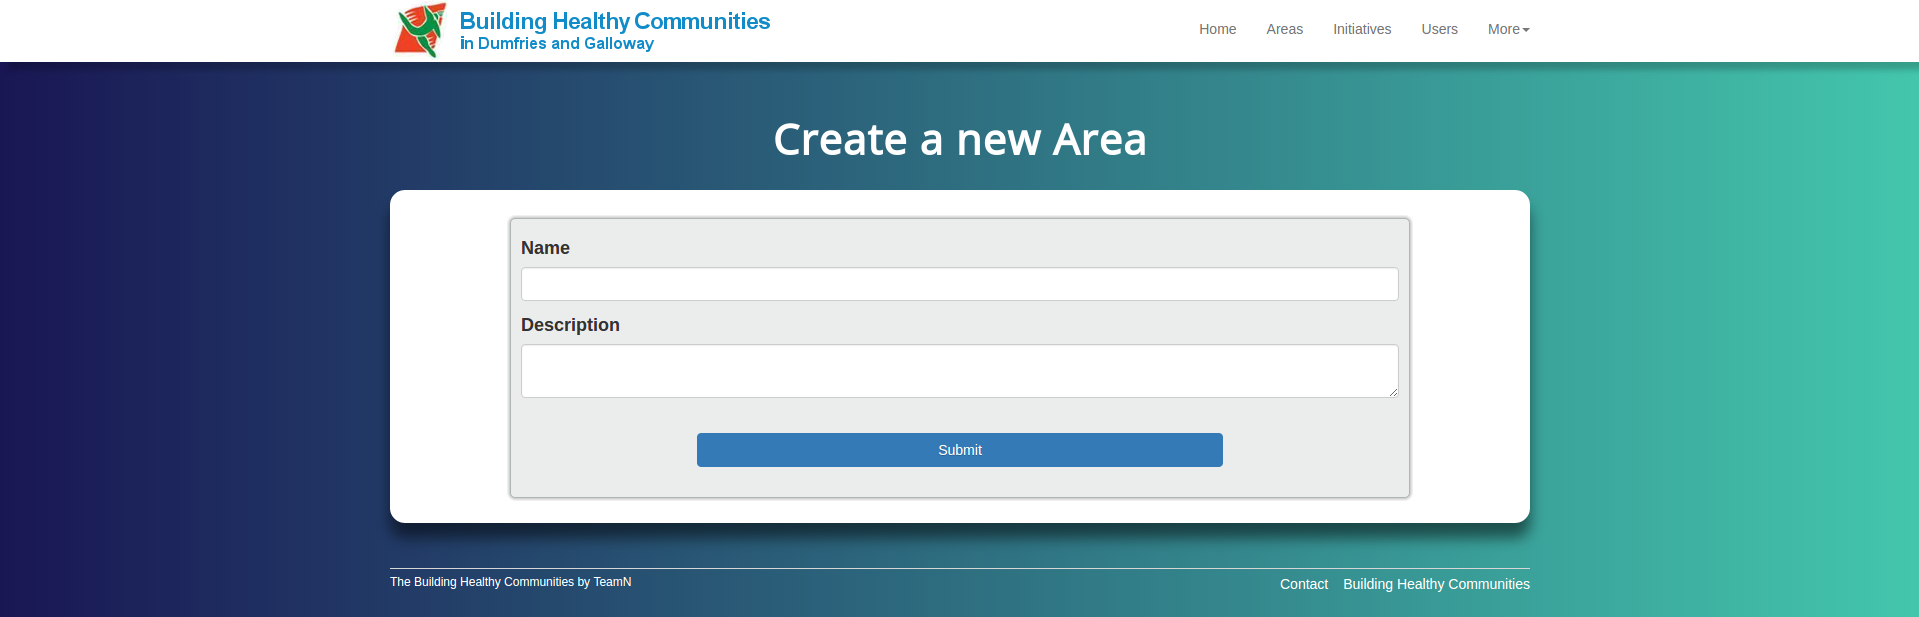
\includegraphics[width=\textwidth, height=\textheight, keepaspectratio]{createarea.png}}
 \caption{Creating an area}
 \label{fig:createArea}
\end{figure}

\section{Initiatives}
\label{sec:initiatives}

Initiatives are the main thrust of the BHC programme, being the events that are run for the benefit of the community. To access the main page of an area, click its name anywhere that it can be found, as with areas. Again, the easiest place to find an initiative name is on the home page or in the Initiatives table.

\subsection{Information and Statistics}
\label{ssec:initinfoandstats}

The main page for an initiative displays all the relevant information about that initiative, laid out in four sections:

\begin{itemize}
	\item The first section contains the initiative's name, a brief description, the date of the last meeting, and the number of enrolled users, and a few other statistics. It also contains a graph of the attendance over time.
	\item The second section contains a table listing all the users enrolled in the initiative. It can be organised by column the same way as the data tables, but not searched.
	\item The third section contains another table, this time listing all meetings of the initiative, both past and scheduled. Again, it can be organised but not searched.
	\item The final section conatins a third table, listing the funding the initiative receives.
\end{itemize}



\subsection{Editing, Deleting and Archiving}
\label{ssec:initeditdelete}

The edit, delete and archive buttons are in the same section as the main statistics, as with areas, but are slightly differently placed.

Editing an initiative allows you to change the name, description and location of an initiative, and also allows you to change the area that initiative belongs to. The editing screen can be seen in \autoref{fig:initEdit}.

Deleting permanently deletes all trace of the initiative from the database, and all users enrolled in it will no longer have it on their enrolment lists. This is a permanent action, deleting actual data, and cannot be undone!

Archiving does not delete the data, but instead places the initiative into the archives. For more on archiving, see \autoref{sec:archives}

\begin{figure}[h!]
 \centerline{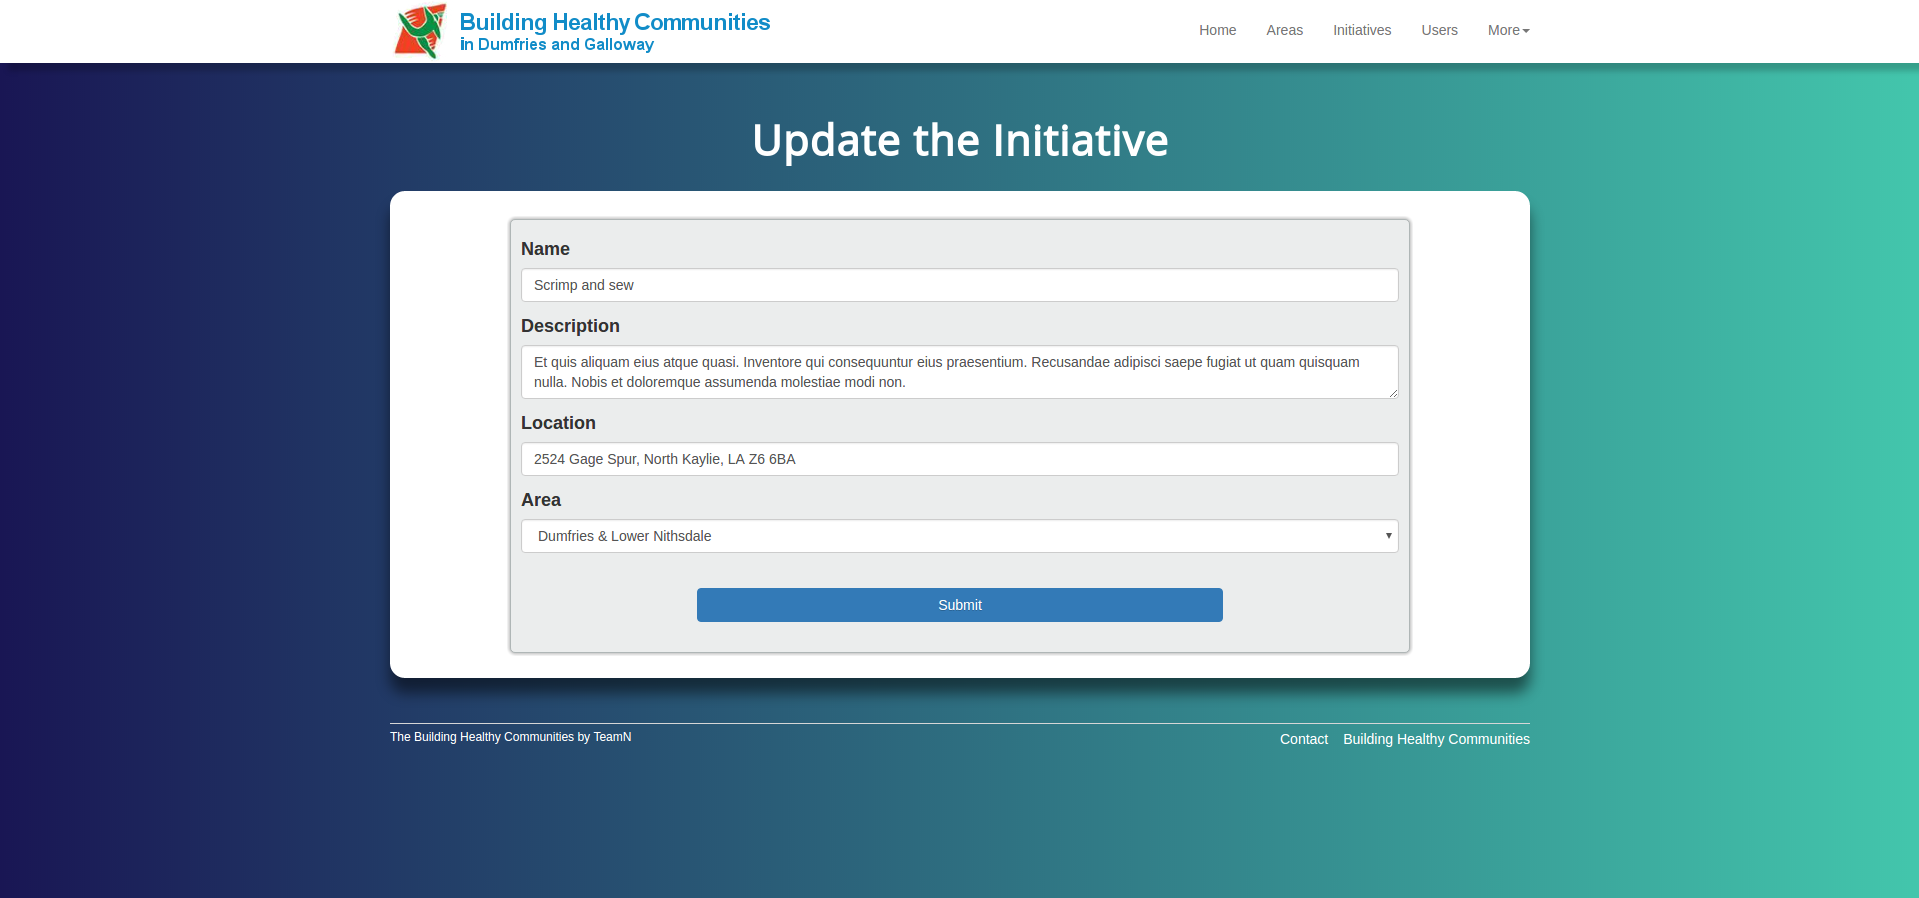
\includegraphics[width=\textwidth, height=\textheight, keepaspectratio]{editinitiative.png}}
 \caption{Editing an initiative}
 \label{fig:initEdit}
\end{figure}

\subsection{Creating a New Initiative}
\label{ssec:createinit}

To create a new initiative, you must click the 'New' button on the Initiatives data table page, as described in \autoref{sec:datatables}: Data Tables, and you will be taken to a short initiative creation screen, as seen in \autoref{fig:createInit}. As with the edit option, adding a name, description, location and area is all that is necessary to create an initiative. The newly created initiative will have no users. To see how to assign users to an area, see the Enrolment and Funding section below.

\begin{figure}[h!]
 \centerline{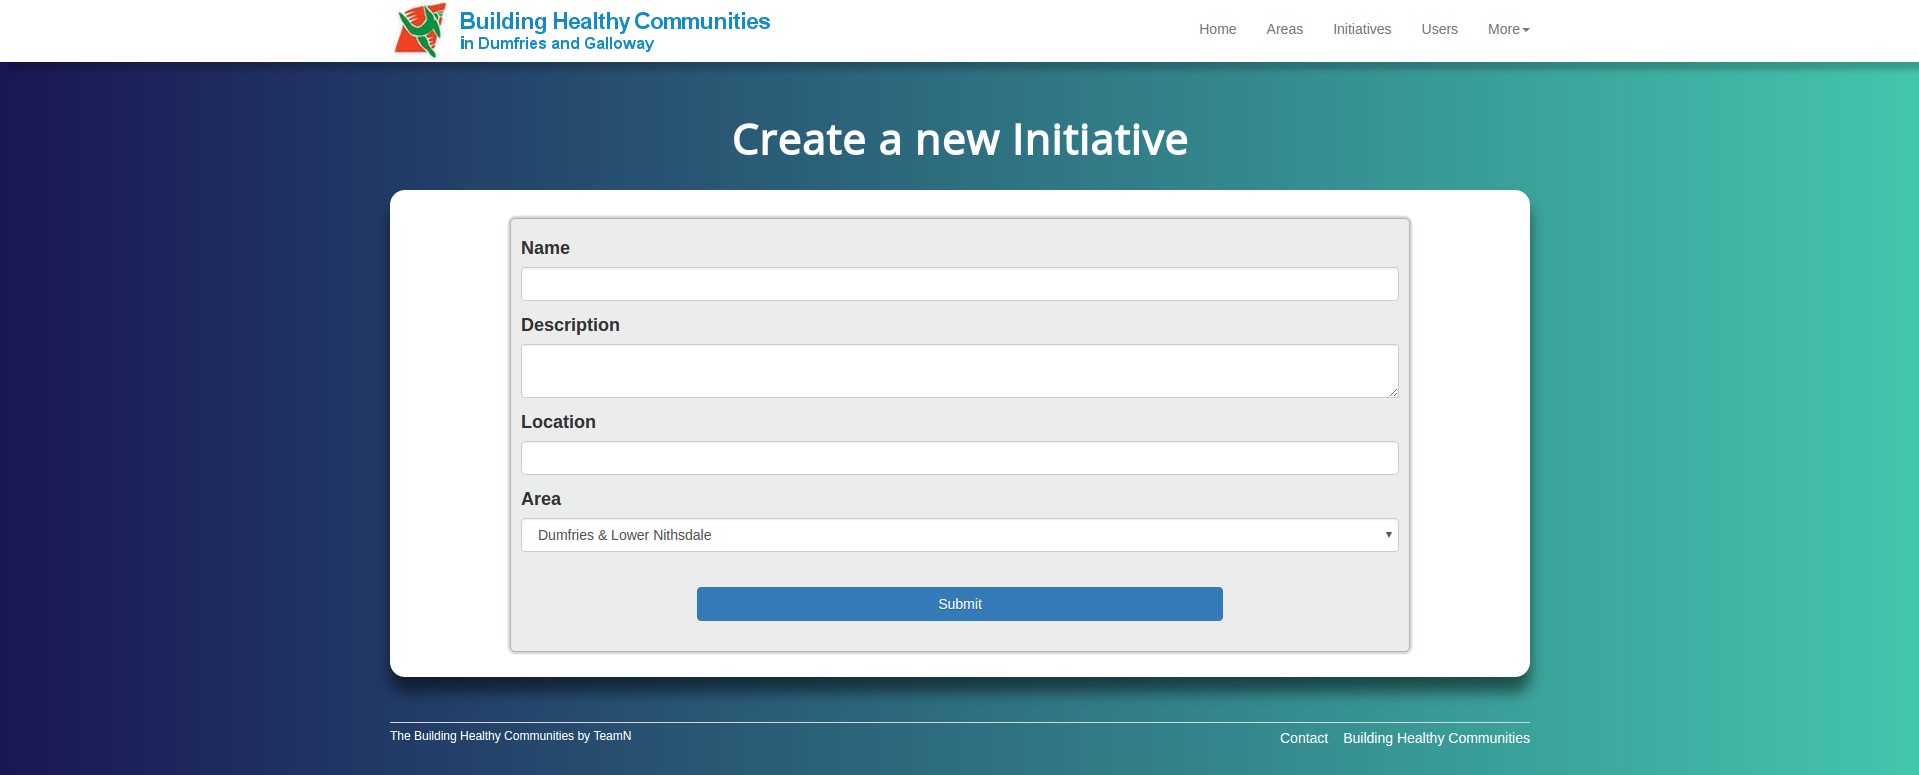
\includegraphics[width=\textwidth, height=\textheight, keepaspectratio]{createinitiative.png}}
 \caption{Creating an initiative}
 \label{fig:createInit}
\end{figure}

\subsection{Enrolment and Funding}
\label{ssec:initenrolfund}

To enrol a new user, simply click the purple 'Enrol' button near the top of the first section of the page, and type in a user's name in the box that appears. Clicking submit will enrol them in the initiative. Unenrolling must be done from the user's page, described in \autoref{sec:users}.

To add new funding, follow a similar procedure to the above, this time selecting the dark green 'Add Funding' button, and selecting a funder from the drop down menu that appears on the next screen. Clicking submit will add them as a funder to the initiative, where they can be viewed at the bottom of the main page, and removed by clikcing the blue 'Remove funding' button.

\subsection{Meetings and Sessions}
\label{ssec:initmeets}

To add a new session, click the green 'New Session' button near the top right of the initiative main page. This will take you to a page titled 'New Meeting', seen in \autoref{fig:initNewSession}. A session is a series of meetings, spaced one week apart but at the same time of day. Use the drop down menus to select the time you want the first meeting to be scheduled for, and the number of weeks you want it to run for. To schedule a single meeting, select 1 week in the 'Weeks to run for' drop down.

For more information on meetings, see \autoref{sec:meetings}: Meetings.

\begin{figure}[h!]
 \centerline{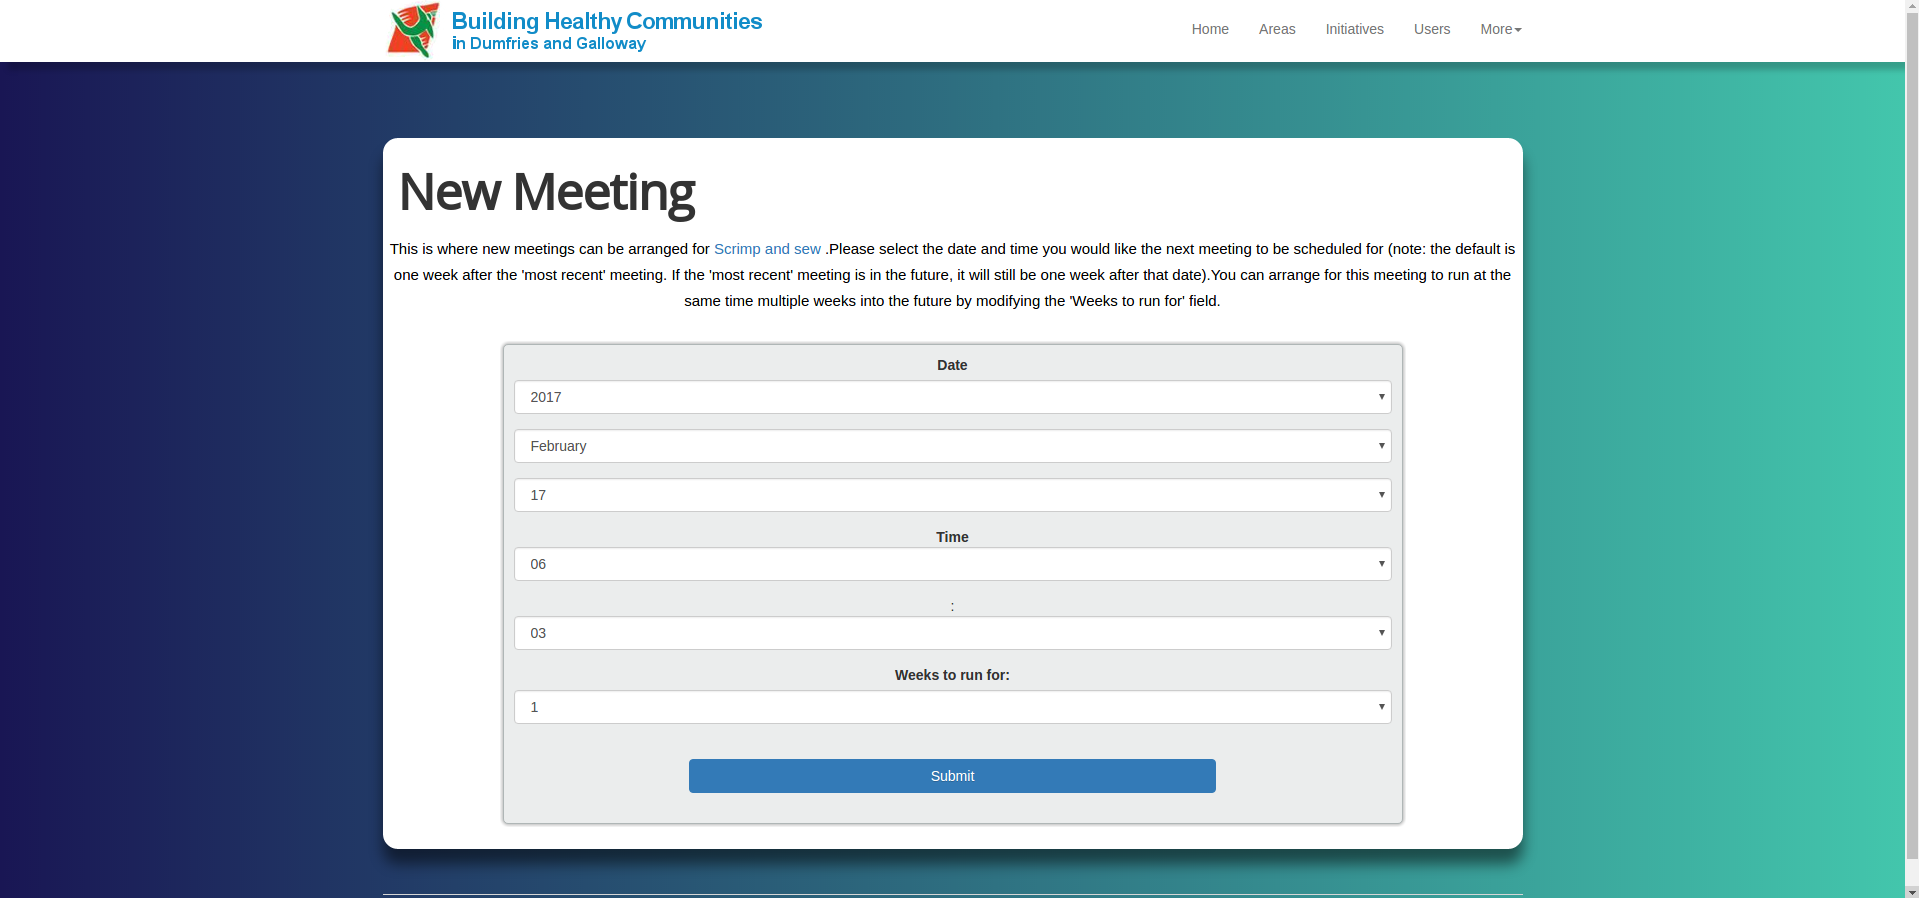
\includegraphics[width=\textwidth, height=\textheight, keepaspectratio]{initnewsession.png}}
 \caption{Creating a new session}
 \label{fig:initNewSession}
\end{figure}

\section{Users}
\label{sec:users}

\subsection{Profile}
\label{ssec:profile}

\section{Medical Conditions}
\label{sec:medical}

\section{Questions}
\label{sec:questions}

\section{Funders}
\label{sec:funders}

\section{Meetings}
\label{sec:meetings}

\section{Archives}
\label{sec:archives}

\section{Contacts and Forgotten Passwords}
\label{sec:contacts}

If you want to find contact details for a given area, there is an easy way to do so. On the login page (you will have to log out if you are currently logged in), in the bottom right is the word 'Contact'. Clicking on this will bring up the contacts page, from which the addresses of the various area partnerships can be found, as seen in \autoref{fig:contactPage}. This page also includes the names and roles of people working there, and a telephone number. If you have forgotten your email address and/or password, then you should contact another administrator directly, as the situation could pose a security risk. Other administrators can reset your account details, but should only do so with your explicit authorisation.

\begin{figure}[h]
 \centerline{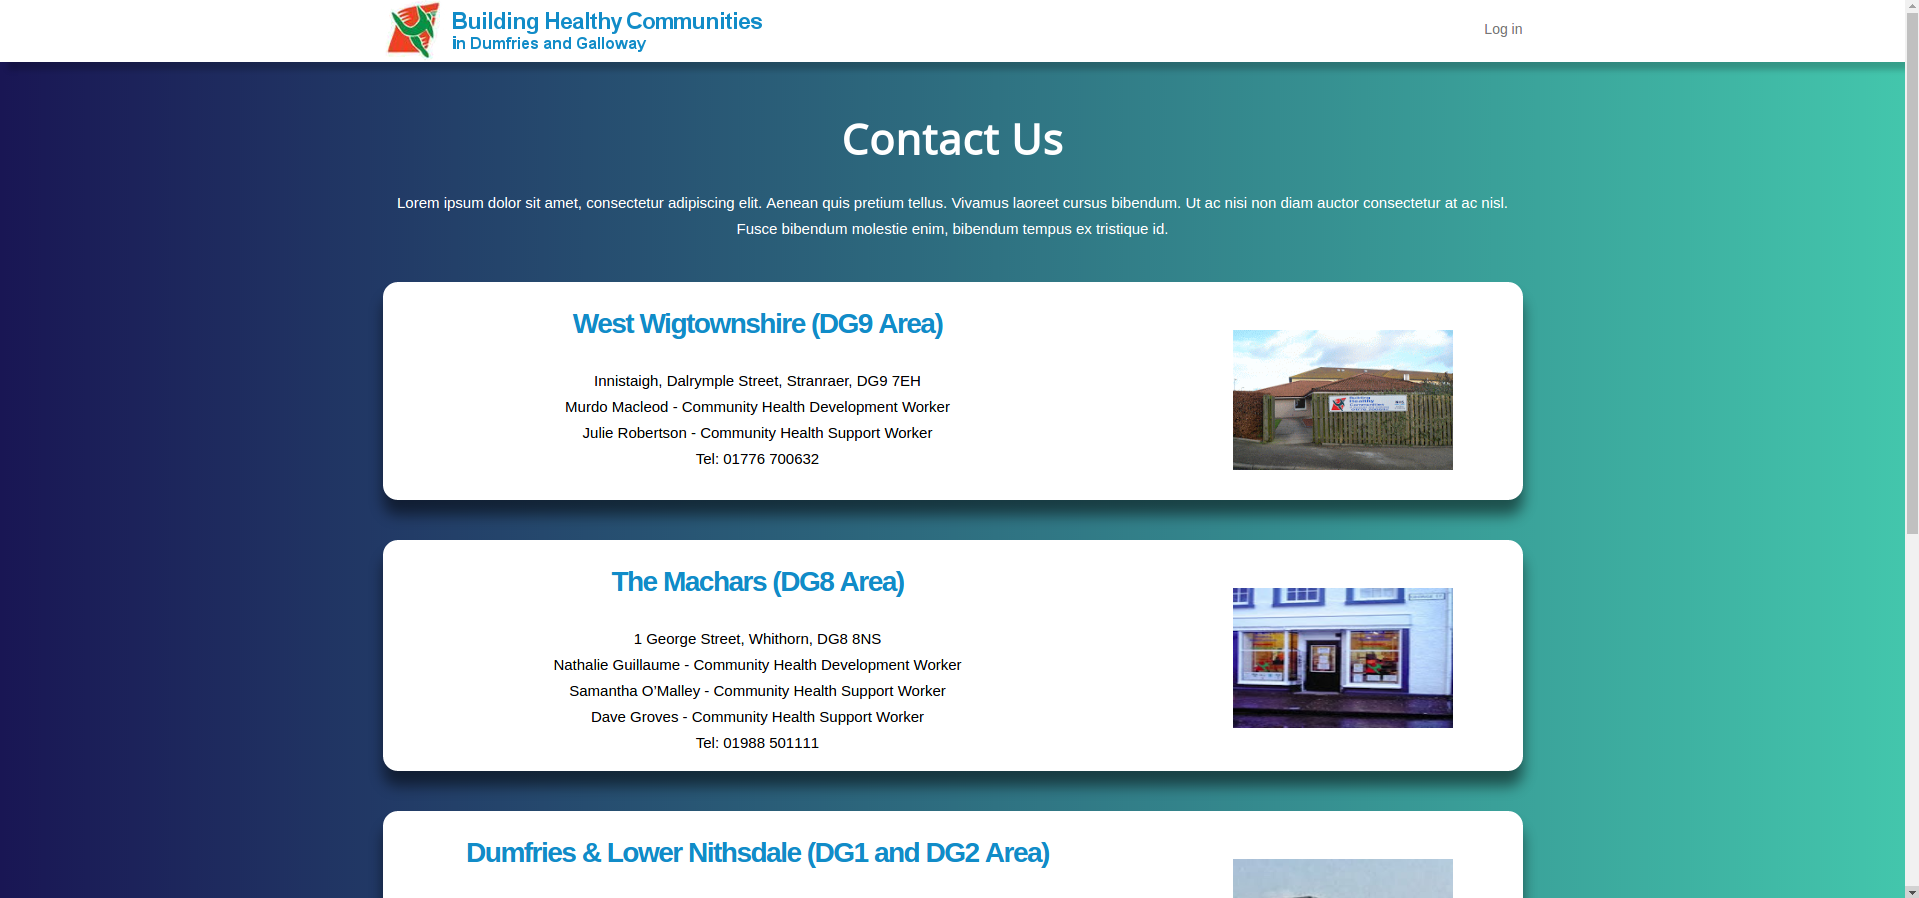
\includegraphics[width=\textwidth, height=\textheight, keepaspectratio]{contactpage.png}}
 \caption{Contact page}
 \label{fig:contactPage}
\end{figure}

\end{document}
